\section{Methodology}
\label{sec:methodology}

This study adopts a comparative experimental design to evaluate two fundamentally different computer vision systems for inspection oriented image analysis. a supervised object detection model YOLOv8 and a multi modal vision-language model LLaVA 1.6. The objective is to compare their ability to detect and identify inspection relevant categories in housing related images under a shared task definition.

This approach addresses a gap in existing research, where supervised detection models and multi modal foundation models are typically evaluated separately, using different datasets, tasks, and metrics. By aligning both models within a single experimental framework, this study enables a controlled comparison of their performance, robustness, and practical applicability.

The methodology describes the experimental procedure and justifies the design choices. Its main contribution lies in the harmonization of fundamentally different model outputs localized detections and textual descriptions—into a shared inspection category space.

\subsection{Research Design}
\label{subsec:research_design}

The research is positioned in the field of computer vision for defect detection and inspection analysis. It follows a comparative experimental design in which two model paradigms are evaluated under identical task conditions:

\begin{itemize}
    \item \textbf{YOLOv8}, a supervised object detection model that produces bounding boxes and class predictions;
    \item \textbf{LLaVA 1.6}, a multi modal vision-language model that generates textual interpretations based on image input and prompts.
\end{itemize}

Both models are applied to the same inspection task and evaluated using a shared category scheme. Their outputs are subsequently aligned to enable direct comparison. This design allows differences in performance to be attributed to the model paradigm rather than to differences in data or evaluation setup.

The novel comparison framework lies in (i) evaluating both models under identical conditions, (ii) introducing a shared inspection oriented label space, and (iii) harmonizing heterogeneous outputs for comparison.

\subsection{Data Sources}
\label{subsec:data_sources}

The experimental setup is based on publicly available datasets obtained through Roboflow, which provide annotated examples of damage related visual patterns

These datasets differ in annotation structure, label definitions, visual characteristics, image quality, and class distributions. They are used as heterogeneous source material for constructing a unified inspection task. 

To enable comparison of the models the original labels are harmonized into a shared set of inspection categories. Figure 1 illustrates the distribution of labels before and figure 2 demonstrates it after harmonization. This process reduces inconsistencies between datasets while preserving the visual diversity required to evaluate model robustness and generalization.

A private housing inspection dataset from DGW is reserved exclusively for application testing. The dataset is not used for training, validation, hyperparameter tuning, or model optimization. Instead, it is used to assess the practical applicability of the developed inspection system within realistic housing inspection workflows. The DGW dataset contains images captured under varying lighting conditions, camera angles, room configurations, occupancy states, and device types, making it suitable for evaluating model performance under real world variability. Consequently, DGW serves as an independent evaluation benchmark rather than a primary training data source during this stage of the research.

The DGW dataset was reserved exclusively for application testing and was not used for training, validation, hyperparameter tuning, or model selection.

\subsection{Dataset Harmonization}
\label{subsec:dataset_harmonization}

The publicly available Roboflow datasets exhibit substantial heterogeneity in annotation structure, label definitions, image composition, and class distributions. Some datasets contain only positive examples, such as the crack detection dataset, while others include both damaged and undamaged images. In addition, identical visual phenomena are often described using different labels across datasets. For example, structural defects may be labeled as \textit{crack}, \textit{damage}, \textit{Amber}, or \textit{Red}, while mold and asbestos datasets use entirely different category schemes.

To enable meaningful comparison, all datasets are harmonized into a shared inspection-oriented label framework consisting of the categories \textit{Damage}, \textit{Wear}, \textit{Mold}, \textit{Asbestos}, and \textit{No Damage}. This harmonization process reduces label inconsistency and ensures that both YOLOv8 and LLaVA are evaluated on the same conceptual inspection task. The complete mapping procedure is shown in Table~\ref{tab:mapping}.

To verify the harmonization procedure, a sample of images from each dataset was manually inspected after label mapping. This validation step was used to confirm that the original labels were consistently assigned to the appropriate harmonized inspection categories. Figure~\ref{fig:harmonization} illustrates the label distribution before and after harmonization, demonstrating how heterogeneous dataset-specific labels were transformed into a unified inspection-category framework.


%------------------------------------
\begin{table}[h]
\caption{Overview of the datasets used in this study.}
\label{tab:datasets}
\centering
\scriptsize
\begin{tabularx}{\columnwidth}{l r X X}
\toprule
Dataset & Images & Original labels & Use \\
\midrule
Asbestos\cite{noauthor_asbestos_nodate} & 932 &
thick-dark-mark, thick-light-mark, thin-dark-mark, thin-light-mark &
Material-mark damage examples \\

Cracks \cite{noauthor_crack_nodate} & 3717 &
crack &
Structural crack examples \\

House Damage \cite{noauthor_house_nodate} & 3008 &
Amber, Green, NoDamage, Red &
General housing damage and no-damage examples \\

Mold \cite{} & 140 &
0, 1, 2 &
Mold-related examples \\

Mold 2 & 938 &
mold &
Mold-related examples \\

Paint Damage & 67 &
Metal &
Paint/surface damage examples \\

Surface Damage & 1665 &
crack, damage, erosion &
Surface deterioration and structural damage examples \\

\bottomrule
\end{tabularx}
\end{table}

%------------------------------------

\begin{figure}[h]
\centering
\includegraphics[width=\columnwidth]{sections/1-thesis-design/original_label_distribution.png}
\caption{Distribution of original dataset labels before harmonization.}
\label{fig:beforeharm}
\end{figure}

\begin{figure}[h]
\centering
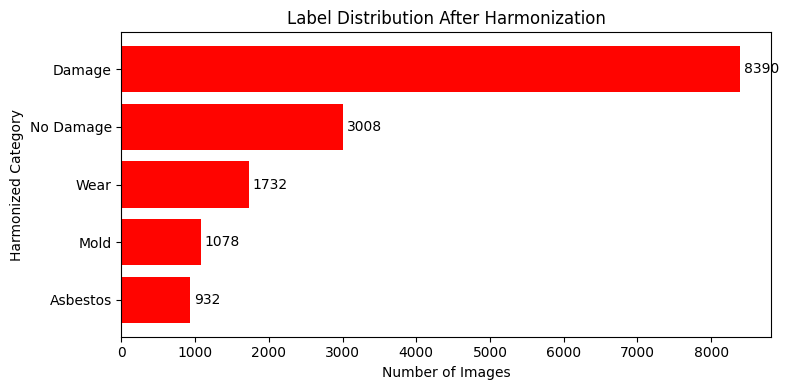
\includegraphics[width=\columnwidth]{sections/2-thesis/harmonizized_label_distribution.png}
\caption{Distribution of harmonized inspection categories after harmonization.}
\label{fig:afterharm}
\end{figure}
%-----------------------------
\begin{table}[h]
\caption{Label harmonization scheme used across datasets.}
\label{tab:mapping}
\centering
\footnotesize
\begin{tabularx}{\columnwidth}{l X}
\toprule
Harmonized Category & Original Labels \\
\midrule
Damage &
crack, damage, Amber, Red \\

Wear &
Metal, erosion \\

Mold &
mold, 0, 1, 2 \\

Asbestos &
thick-dark-mark, thick-light-mark,
thin-dark-mark, thin-light-mark \\

No Damage &
NoDamage, Green \\
\bottomrule
\end{tabularx}
\end{table}

%--------------------------------
\subsection{Inspection Categories}
\label{subsec:inspection_categories}

The shared label scheme consists of four inspection-relevant categories:

\begin{itemize}
    \item \textbf{Damage}: structural or material damage such as cracks, holes, or breakage;
    \item \textbf{Wear}: gradual deterioration such as discoloration or surface aging;
    \item \textbf{Alteration}: visible modification or deviation from the intended structure;
    \item \textbf{No damage}: absence of inspection-relevant issues.
\end{itemize}

This schema is derived from the application domain rather than from the original dataset labels. All source labels are mapped to these categories where possible. Labels that do not align clearly are excluded or treated cautiously during interpretation.

\subsection{Dataset Bias and Limitations}

The public datasets used in this study originate from different domains and collection procedures, introducing variation in image composition, annotation practices, and class distributions. For example, crack datasets primarily contain close up defect images, whereas housing inspection datasets contain wider room level views.

Class imbalance is another limitation, as some categories, such as paint damage, contain substantially fewer examples than others.

Consequently, the results should be interpreted within the context of the selected datasets and the harmonized inspection framework used in this study.

\subsection{Pipeline Model}
\label{subsec:pipeline_model}

The experimental setup is organized as a unified pipeline model that enables a controlled comparison between YOLOv8 and LLaVA 1.6. Rather than evaluating both models independently, they are embedded in the same processing framework consisting of four main stages: data preparation, parallel model execution, output harmonization, and evaluation. This structure ensures that differences in performance can be attributed to the model paradigms themselves rather than to inconsistencies in data handling or evaluation design.

%--------------------------------------

```latex
\begin{figure}[h]
\centering
\fbox{\parbox{0.9\columnwidth}{\centering
Public Datasets\\
(Training Data)
}}

\vspace{0.2cm}
$\downarrow$

\vspace{0.2cm}
\fbox{\parbox{0.9\columnwidth}{\centering
Dataset Harmonization
}}

\vspace{0.2cm}
$\downarrow$

\vspace{0.2cm}
\fbox{\parbox{0.9\columnwidth}{\centering
YOLOv8 \hspace{1cm} LLaVA 1.6
}}

\vspace{0.2cm}
$\downarrow$

\vspace{0.2cm}
\fbox{\parbox{0.9\columnwidth}{\centering
Unified Inspection Categories
\\
(Damage, Wear, Mold, Asbestos, No Damage)
}}

\vspace{0.2cm}
$\downarrow$

\vspace{0.2cm}
\fbox{\parbox{0.9\columnwidth}{\centering
Evaluation on DGW Test Set
}}

\caption{Overview of the experimental pipeline.}
\label{fig:pipeline}
\end{figure}
```

%-------------------------------------

Figure~\ref{fig:pipeline} shows the overall pipeline model used in this study. The process starts with publicly available Roboflow datasets, which are first harmonized into a shared inspection category scheme. The prepared data is then used in two parallel branches. In the first branch, YOLOv8 is trained on the harmonized annotated data and applied to test images to produce structured detections. In the second branch, LLaVA 1.6 processes the same test images using fixed prompts and generates textual descriptions. Because these outputs are fundamentally different, they are subsequently transformed into a shared image-level representation through a rule-based harmonization step. The aligned outputs are then evaluated using both detection and classification metrics, supported by confusion matrices and qualitative error analysis.

This pipeline model is central to the methodology because it operationalizes the comparison between supervised detection and multi modal reasoning within a single consistent framework.


```latex
\subsection{Experimental Setup}
\label{subsec:experimental_setup}

The experimental setup was designed to ensure a fair comparison between YOLOv8 and LLaVA 1.6 under identical inspection conditions. All public datasets were harmonized into a shared inspection-category framework consisting of Damage, Wear, Mold, Asbestos, and No Damage. The DGW dataset was excluded from model training and reserved exclusively for application testing.

\subsubsection{Data Preparation}

The harmonized dataset was divided into training, validation, and test subsets using a stratified split. A ratio of 70\% training, 15\% validation, and 15\% testing was applied. All annotations were represented as bounding boxes. Images from the DGW dataset were not used for training, validation, hyperparameter tuning, or model selection.

\begin{table}[h]
\caption{Experimental configuration.}
\label{tab:experimental_setup}
\centering
\footnotesize
\begin{tabularx}{\columnwidth}{l X}
\toprule
Setting & Value \\
\midrule
YOLO Model & YOLOv8m \\
Pretrained Weights & COCO-pretrained weights \\
Image Size & 640 $\times$ 640 \\
Epochs & 75 \\
Batch Size & 32 \\
Patience & 20 \\
Random Seed & 42 \\
Workers & 24 \\
Train/Validation/Test Split & 70/15/15 \\
LLaVA Model & LLaVA v1.6 Mistral 7B \\
Inference Mode & Zero-shot \\
Prompt Strategy & Fixed prompt template \\
Output Mapping & Rule-based category mapping \\
\bottomrule
\end{tabularx}
\end{table}

\subsubsection{Model Configuration}

YOLOv8 was trained using the harmonized training dataset and initialized with pretrained COCO weights. The model was trained for 75 epochs using a fixed random seed to support reproducibility. Hyperparameters were kept constant throughout the experiments.

LLaVA 1.6 was evaluated in a zero-shot setting without task-specific training. The model received the same prompt for all images to ensure consistency across evaluations. Generated textual outputs were converted to the harmonized inspection categories using a predefined rule-based mapping procedure.

The prompt used during evaluation was:

\begin{quote}
Choose exactly one category from the following list: Damage, Wear, Mold, Asbestos, or No Damage. Respond using only the category name.
\end{quote}

\subsubsection{Evaluation Procedure}

Both models were evaluated using the same inspection categories and test images. YOLOv8 predictions were evaluated using object-detection metrics, while LLaVA outputs were evaluated after conversion to the shared inspection categories. This approach ensured that both models were compared on the same inspection task despite their different output formats.

Figure~\ref{fig:pipeline} provides an overview of the experimental workflow.
```


\subsubsection{Data preparation}

The datasets are first processed by mapping their original labels to the shared inspection categories. Where necessary, labels are merged or reinterpreted to ensure consistency. The resulting dataset is then formatted for model input.

For YOLOv8, the data is divided into training, validation, and test sets using a stratified split of 70\%, 15\%, and 15\%, where feasible. This ensures that class distributions are preserved across splits.

For LLaVA, the test images are used directly without additional preprocessing beyond standard input formatting.

\subsubsection{YOLOv8 training}

YOLOv8 is trained on the harmonized dataset using pretrained weights. Training is performed with fixed hyper parameters to ensure reproducibility and comparability. These include the number of epochs, batch size, input resolution, learning rate, and detection thresholds.

The final model is selected based on validation performance and evaluated on the test set.

\subsubsection{LLaVA inference}

LLaVA 1.6 is applied in inference mode using fixed prompt templates. Each image is evaluated using the same prompts to ensure consistency and avoid bias. Example prompts include:

\begin{itemize}
    \item ``Identify visible damage in this image.''
    \item ``Is there evidence of wear or alterations in this image?''
\end{itemize}

No fine-tuning is performed, as the goal is to assess zero-shot performance in an inspection context.

\subsubsection{Output harmonization}

YOLOv8 produces bounding boxes with class predictions, while LLaVA produces textual descriptions. To enable comparison, both outputs are mapped to the shared inspection categories.

For YOLOv8, detections below a confidence threshold are removed, and remaining detections are aggregated to image-level category predictions.

For LLaVA, textual outputs are converted into category labels using a predefined keyword-based mapping scheme. Ambiguous cases are flagged for qualitative analysis.

This harmonization step is central to the methodology, as it enables direct comparison between fundamentally different output formats.

\subsection{Evaluation Metrics}
\label{subsec:evaluation_metrics}

Evaluation is performed using both detection and classification metrics.

For YOLOv8, performance is measured using:

\begin{itemize}
    \item Precision
    \item Recall
    \item mean Average Precision (mAP)
\end{itemize}

For the shared comparison between models, image level classification metrics are used:

\begin{itemize}
    \item Accuracy
    \item Precision
    \item Recall
    \item F1-score
\end{itemize}

Confusion matrices are used to analyze category-level errors and misclassifications.

\subsection{Reproducibility}

Experiments use fixed seeds where applicable to support reproducibility. Dataset preprocessing, harmonization procedures, inference settings, and evaluation pipelines are version controlled through GitHub. Public datasets and experimental configurations are documented to enable replication.

\subsection{Qualitative Analysis}
\label{subsec:qualitative_analysis}

To complement quantitative evaluation, a qualitative analysis is conducted on representative examples. Misclassifications and ambiguous predictions are examined to identify recurring failure modes, such as subtle damage, visual clutter, or unclear model interpretations.

\subsection{Validity, Reliability, and Reproducibility}
\label{subsec:validity_reliability}

Internal validity is ensured by evaluating both models under identical conditions, using fixed prompts and consistent training settings. Construct validity is supported by aligning all data and outputs to inspection-relevant categories.

Reliability is supported through consistent preprocessing, fixed configurations, and documented procedures. Reproducibility is ensured by implementing the pipeline in Python and reporting all relevant settings.

\subsection{Ethical Considerations}
\label{subsec:ethical_considerations}

The experiments are conducted on publicly available datasets in a controlled research setting. The study is intended as decision-support research and does not replace human inspection judgment.

\subsection{Error Analysis}

Model failures are categorized into error types including missed detections, false detections, category confusion, robustness failures under environmental variation, and output harmonization failures. Qualitative analysis complements quantitative evaluation.